\documentclass{article}
\usepackage{graphicx} % Required for inserting images
\usepackage{listings}

\lstset{language=Python, numbers=left}

\title{Labwork 2: Hello, CUDA!}
\author{Phi Doan Minh Luong - 2440046}
\date{September 2025}

\begin{document}

\maketitle

\setlength\parindent{0pt}

\section{Preprocessing}
We will use the Lenna image for this labwork.
\begin{figure}[h]
    \centering
    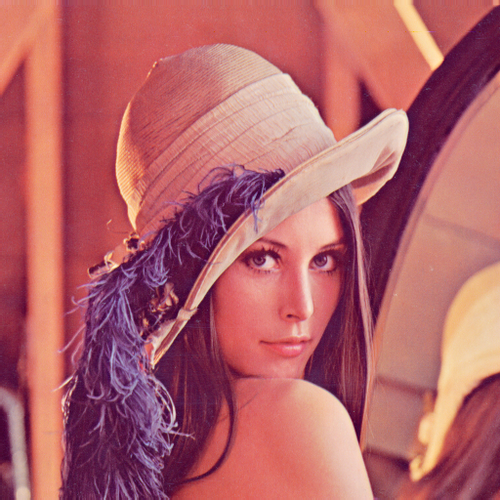
\includegraphics[width=0.5\linewidth]{Lenna.png}
\end{figure}

We load the image using the OpenCV library, then flatten the image into a 1D array of RGB values using the Numpy library

\begin{lstlisting}
rgb = cv2.imread("Lenna.png")
imageHeight, imageWidth, _ = rgb.shape
print(imageHeight, imageWidth)
pixelCount = imageHeight * imageWidth
rgb = np.reshape(rgb, (pixelCount, 3))
print(rgb.shape)
\end{lstlisting}

\section{CPU}
We implement grayscale using the CPU
\begin{lstlisting}
def grayscale_cpu(src, dst):
  for i in range(pixelCount):
    g = np.uint8((int(src[i, 0]) + int(src[i, 1]) + int(src[i, 2])) / 3)
    dst[i, 0] = dst[i, 1] = dst[i, 2] = g
  return dst
\end{lstlisting}

The average processing time after running 10 times is 0.4067821502685547 seconds. The resulting image is:
\begin{figure}[h]
    \centering
    
\includegraphics[width=0.5\linewidth]{Lenna_gray_cpu.png}
\end{figure}

\section{GPU}
First, we defined a function to convert an image to grayscale on the GPU. 
\begin{lstlisting}
@cuda.jit
def grayscale_gpu(src, dst):
  tidx = cuda.threadIdx.x + cuda.blockIdx.x * cuda.blockDim.x
  g = np.uint8((src[tidx, 0] + src[tidx, 1] + src[tidx, 2]) / 3)
  dst[tidx, 0] = dst[tidx, 1] = dst[tidx, 2] = g
\end{lstlisting}

Then, we follow the flow of the CUDA program, calculate the average time processed after running each block size 10 times
\begin{lstlisting}
devOutput = cuda.device_array((pixelCount, 3), np.uint8)
devInput = cuda.to_device(rgb)
blockSize = [32, 64, 128, 256, 512, 1024]
timeProcess = []

for b in blockSize:
  gridSize = math.ceil(pixelCount / b)
  avgtime = []
  for _ in range(10):
    start = time.time()
    grayscale_gpu[gridSize, b](devInput, devOutput)
    avgtime.append(time.time() - start)
    hostOutput = devOutput.copy_to_host()
    grayscale_gpu_image = hostOutput.reshape((imageHeight, imageWidth, 3))
  cv2.imwrite(f"Lenna_gray_gpu_{b}.png", grayscale_gpu_image)
  timeProcess.append(np.mean(avgtime))
  print(f"Time processed with block size {b}: {np.mean(avgtime)}s")
\end{lstlisting}

The resulting images are all the same. The average time results are:
\begin{lstlisting}
Time processed with block size 32: 0.0002749919891357422s
Time processed with block size 64: 0.00018134117126464844s
Time processed with block size 128: 0.00011363029479980469s
Time processed with block size 256: 0.00012094974517822266s
Time processed with block size 512: 0.0001163482666015625s
Time processed with block size 1024: 0.000121307373046875s
\end{lstlisting}

Here, I plot a graph of block size vs time
\begin{figure}[h]
    \centering
    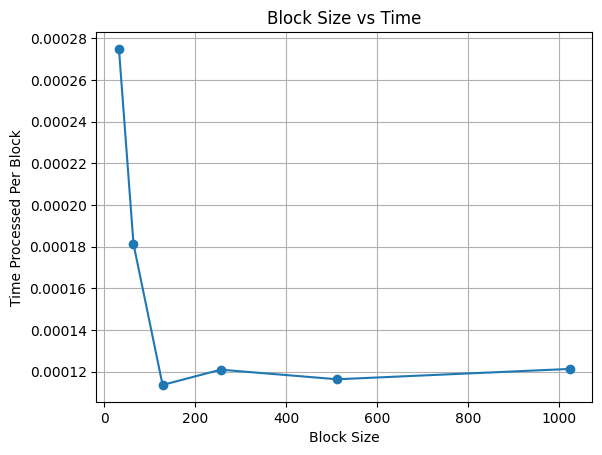
\includegraphics[width=0.8\linewidth]{blocksize.png}
\end{figure}

At the small block sizes (32 and 64), the processing time per block is higher. This is because small block sizes may not fully utilize the GPU, leading to a higher time per block.

At the optimal block sizes (128 to 512), it used threads and cores more efficiently, reducing the processing time.

At the high block size (1024), there is a slight increase in processing time.

\end{document}
